\documentclass[border=5pt,convert={outfile=../_static/\jobname.svg}]{standalone}

\usepackage{tikz}

\begin{document}

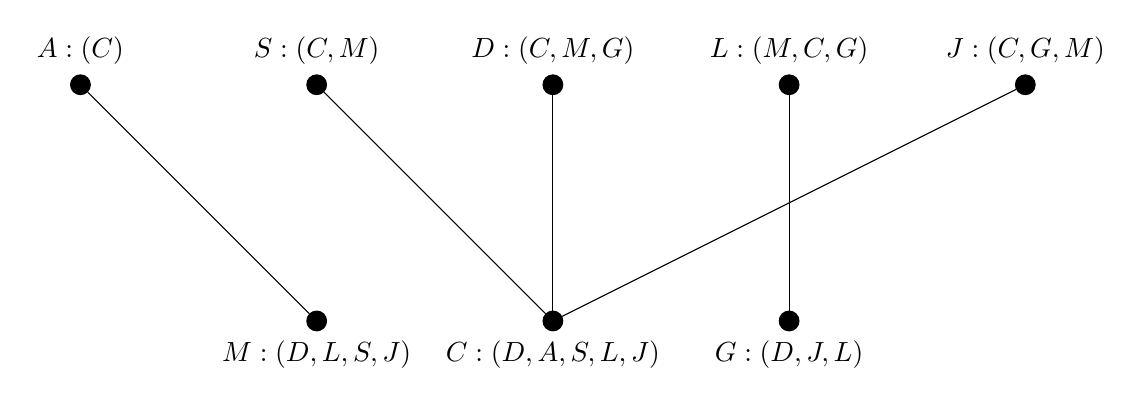
\begin{tikzpicture}[scale=0.5]

    % Residents
    \node[draw, shape=circle, fill, inner sep=0, minimum size=0.25cm,
    label=above: {\(A: (C)\)}] (A) at (0, 0) {};
    \node[draw, shape=circle, fill, inner sep=0, minimum size=0.25cm,
    label=above: {\(S: (C, M)\)}] (S) at (6, 0) {};
    \node[draw, shape=circle, fill, inner sep=0, minimum size=0.25cm,
    label=above: {\(D: (C, M, G)\)}] (D) at (12, 0) {};
    \node[draw, shape=circle, fill, inner sep=0, minimum size=0.25cm,
    label=above: {\(J: (C, G, M)\)}] (J) at (24, 0) {};
    \node[draw, shape=circle, fill, inner sep=0, minimum size=0.25cm,
    label=above: {\(L: (M, C, G)\)}] (L) at (18, 0) {};

    % Hospitals
    \node[draw, shape=circle, fill, inner sep=0, minimum size=0.25cm,
    label=below: {\(M: (D, L, S, J)\)}] (M) at (6, -6) {};
    \node[draw, shape=circle, fill, inner sep=0, minimum size=0.25cm,
    label=below: {\(C: (D, A, S, L, J)\)}] (C) at (12, -6) {};
    \node[draw, shape=circle, fill, inner sep=0, minimum size=0.25cm,
    label=below: {\(G: (D, J, L)\)}] (G) at (18, -6) {};

    % Lines
    \foreach \x in {S, D, J}
        \draw (\x) -- (C);

    \draw (A) -- (M);
    \draw (L) -- (G);

\end{tikzpicture}

\end{document}
